\documentclass[a4paper, 12pt]{article}

\usepackage[utf8]{inputenc}

\usepackage{graphicx}
\usepackage{wrapfig}
\usepackage{caption}
\usepackage{parskip}

\usepackage{physics}
\usepackage{amsmath}

\usepackage{tikz}
\usepackage{tkz-graph}
\usepackage{tikzscale}
\usetikzlibrary{arrows}

\captionsetup{width=0.8 \linewidth}

\usepackage{hyperref}

\begin{document}

\title{\vspace{-6em}\textbf{Homework 5}\\ \Large Information Theory for Complex Systems \vspace{-3.2em} }
\author{} \date{March - 2023}

\maketitle

\pagenumbering{gobble}

\section*{a)}
In order to show that $A = [0, 0.5], B = (0.5,1]$ is a generative partition we need to show that diam$(x_1 x_2 \dots x_m) \rightarrow 0$ as $m \rightarrow 0$ as we consider sequences of increasing length.

\begin{wrapfigure}{r}{5.5cm}
    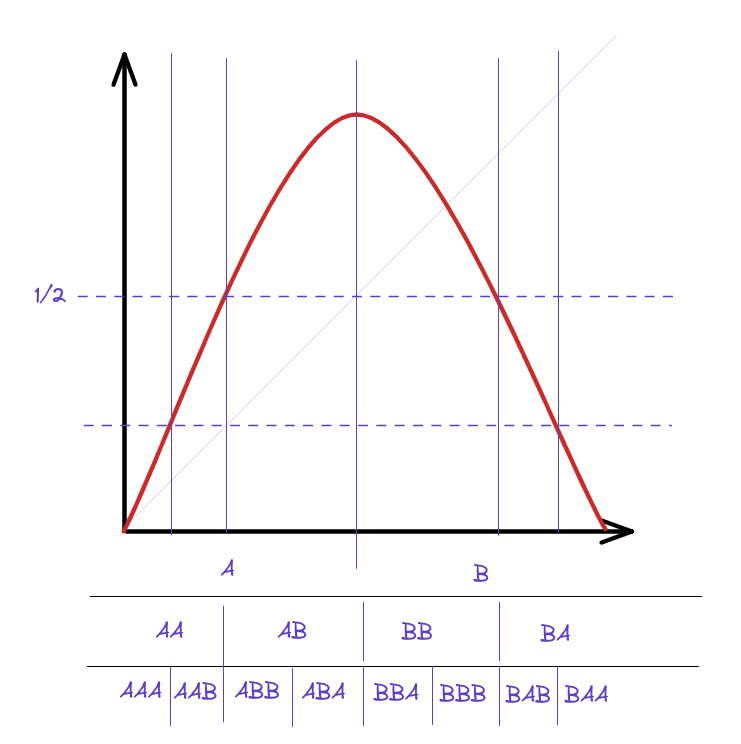
\includegraphics[width=\linewidth,trim={0 2cm 0 2cm}]{map.png}
\end{wrapfigure}

As can be seen in the figure to the right, whenever we add another symbol to the sequence each interval is split into two subsets. As we can observe, there's always one subset with an $A$ added at the end and one with a $B$ at the end. The partition therefore enumerates all permutations of $A$ and $B$ uniquely. We get no disconnected sets, therefore all new splits shrink in size, equivalent with diam$(x_1 x_2 \dots x_m) \rightarrow 0$ as $m \rightarrow 0$.

\section*{b)}
Starting at $x_0 = 0.2$, iterating the logistic map for 100\,000 steps results in $P(A) = 0.51$ and $P(B) = 0.49$.

\section*{c)}
I use the given ergodic measure and plug it into equation (8.6) from the course book which gives
\begin{equation}
    \lambda = \int \mu(x) \ln |f'(x)| dx = \int_0^1 \frac{\ln |4((1 - x) - x)|}{\pi \sqrt{x (1-x)}} dx = \ln 2,
\end{equation}
which I calculated in Mathematica.

\section*{d)}
Reading the time series and calculating the probabilities using the original $A$ and $B$ results in $P(A) = 0.36$ and $P(B) = 0.64$). This asymmetry doesn't match up at all with the simulated results. Switching the partition to $A' = [0.324, 0.6004]$ and $B' = (0.7884864, 0.9]$ results in $P(A') = 0.50$ and $P(B') = 0.50$.


\section*{Appendix: Source Code}
All code is additionally availible at \url{https://github.com/vincent-uden/tif150-information-theory-for-complex-systems}
\begin{figure}[ht!]
    \centering
    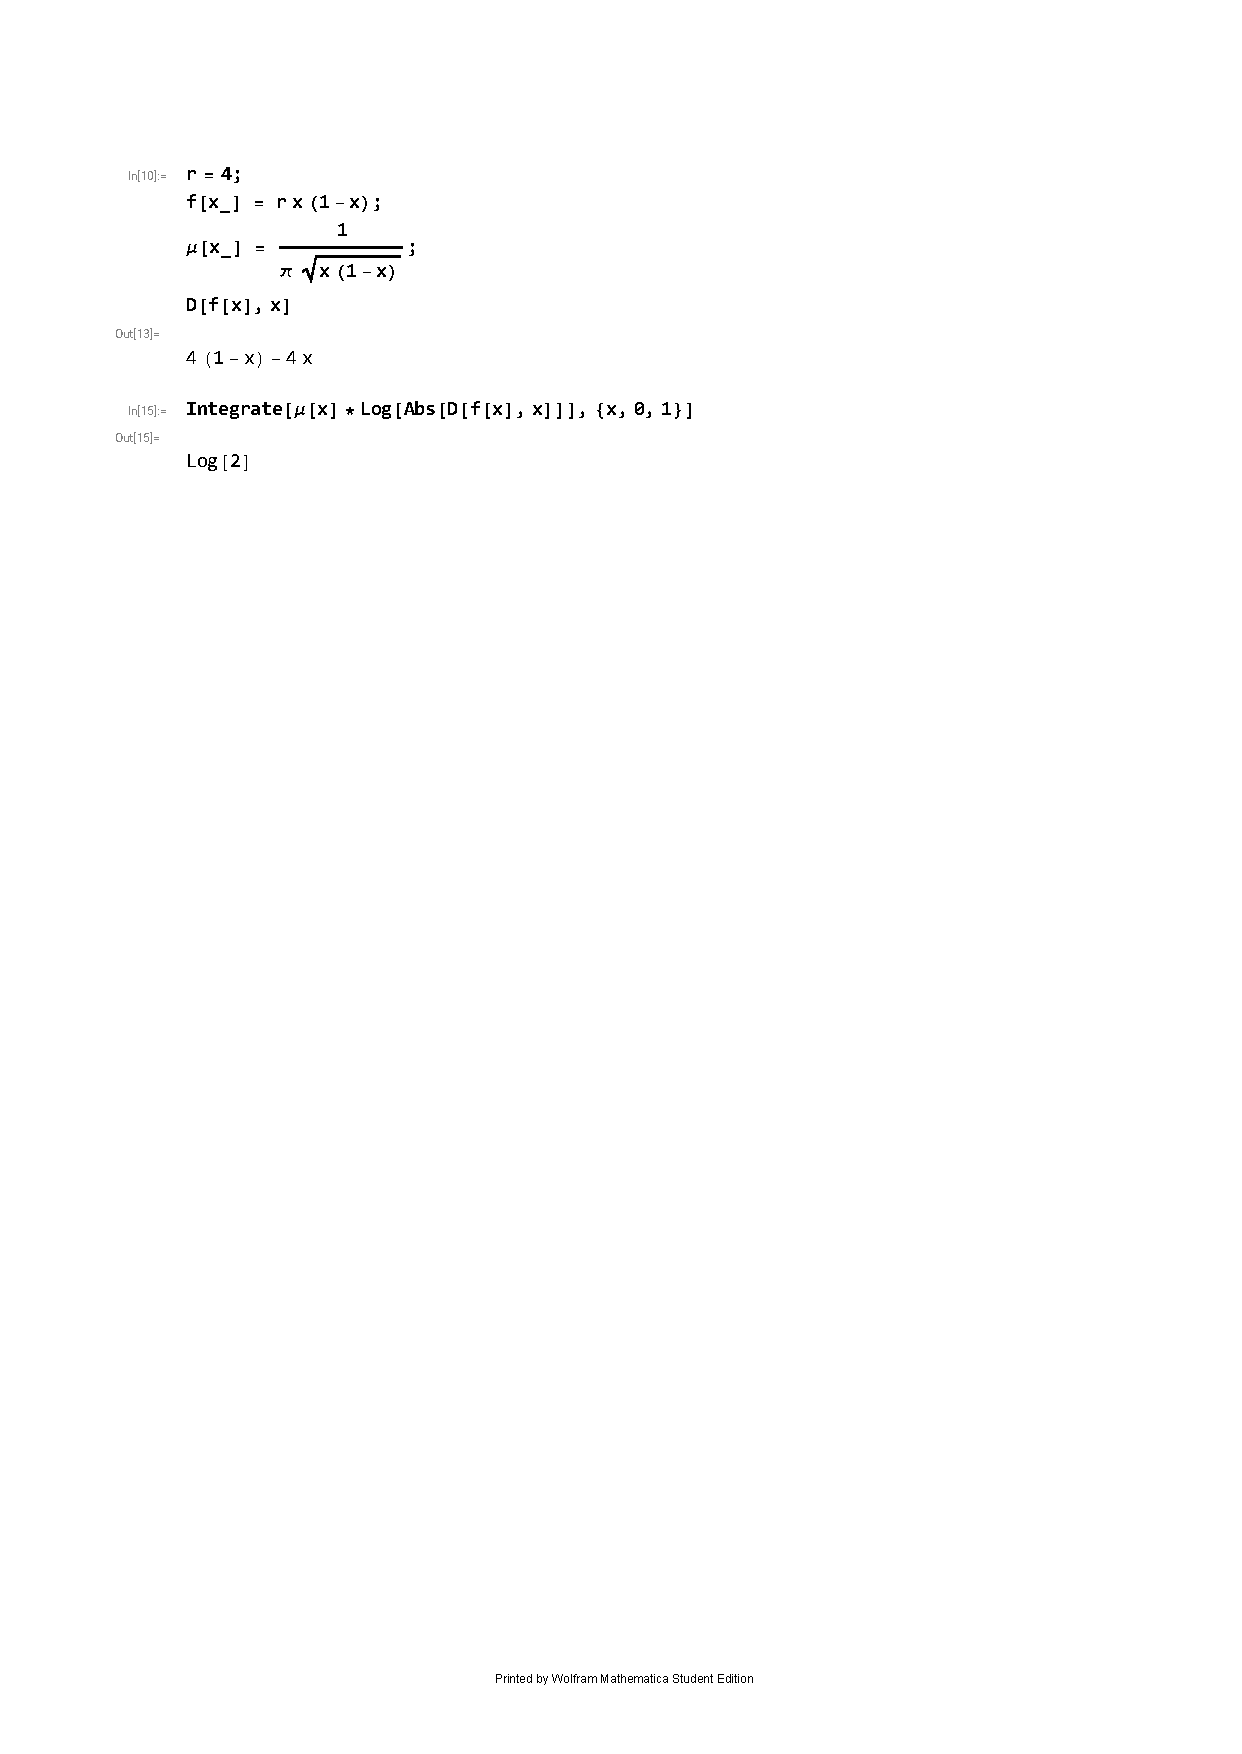
\includegraphics[trim={2cm 20cm 2cm 2cm}]{../../src/integral.pdf}
\end{figure}


\end{document}
